\documentclass[11pt]{beamer}
\usepackage{verbatim}
\usepackage{amsmath}
\usepackage{amsthm}
\usepackage{multicol}
\usepackage{graphics}
\usepackage{color}
\usepackage{stmaryrd}\usefonttheme[onlymath]{serif}

\title{Termination Analysis for Multi-Path Linear Loops}
\date{\today}
\author{Hui Jin et. al from Tianjin Uni.}


\begin{document}
\maketitle

\begin{frame}\frametitle{History of Research}
Joint research with Xiaofei Xie of NTU.

\begin{itemize}

\item Xiaofei Xie, Bihuan Chen, Liang Zou, Shang-Wei Lin, Yang Liu, and Xiaohong Li. “Loopster: static loop termination analysis.” In Proceedings of the 2017 11th Joint Meeting on Foundations of Software Engineering, pp. 84-94. ACM, ESEC/FSE 2017
\item Xiaofei Xie, Bihuan Chen, Liang Zou, Yang Liu, Wei Le, and Xiaohong Li. X. Xie, B. Chen, L. Zou, Y. Liu, W. Le and X. Li, “Automatic Loop Summarization via Path Dependency Analysis.” In IEEE Transactions on Software Engineering, vol. 45, no. 6, pp. 537-557, TSE 2019
\end{itemize}
\end{frame}
\begin{frame}\frametitle{Contribution}
\begin{itemize}
\item Extend the path dependency automaton(PDA) to analyze the linear loop and extract paths in CFG as states in the PDA to obtain the dependecy relationship between paths.

\item Make a simple classification of cycles in PDA, and proposed methods to determie the termination of the cycle.

\item Implement algorithm proposed by Tiwari to determine the termination of linear loops. 
\end{itemize}
\end{frame}

\begin{frame}\frametitle{Control Flow Graph and Path}
\begin{definition}[Control Flow Graph(CFG)]
A control flow graph of a loop is a tuple $\mathcal{G} = (V,E,v_s, V_h, V_e, \i)$, where $V_h, V_e$ are the set of header blocks and exit blocks respectively. $\i(e)$ is the branch conditio nof the edge $e\in E$.

\end{definition}

\begin{definition}\frametitle{Loop Path of CFG}
Given a CFG $\mathcal{G} = (V,E,v_s, V_h, V_e, \i)$, the loop path $\sigma$ is a finite sequence $v_0,v_1, \ldots, v_k$ of basic blocks where $v_0 \in V_h$ and $v_k\in V_h\cup V_e$ are the head and tail of $\sigma$. We call a path iterable path if $head(\sigma) = tail(\sigma)$.

\begin{itemize}
\item Path condition: $\theta_\sigma$ is the conjunction of the branch condition of each edge in the path.
\item Value change of vars: $\mathcal{V}_\sigma$. $\theta(\sigma_i, \mathcal{V}^n_{\sigma_j})\rightarrow \{true, false\}$.
\item $pre(\mathcal{G})$: precondition of loop represent the possible valuation of vars.	
\end{itemize}
\end{definition}
\end{frame}

\begin{frame}\frametitle{Exmaple}
\begin{center}
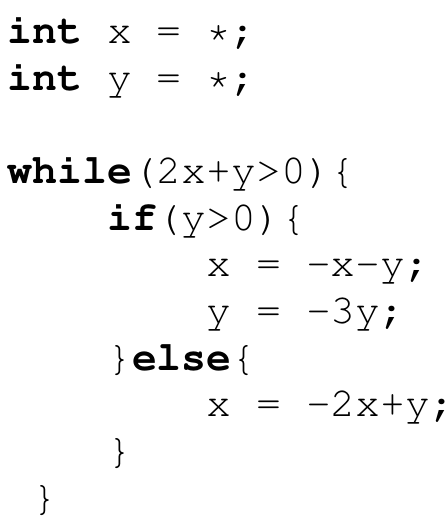
\includegraphics[scale=0.25]{1code.png}
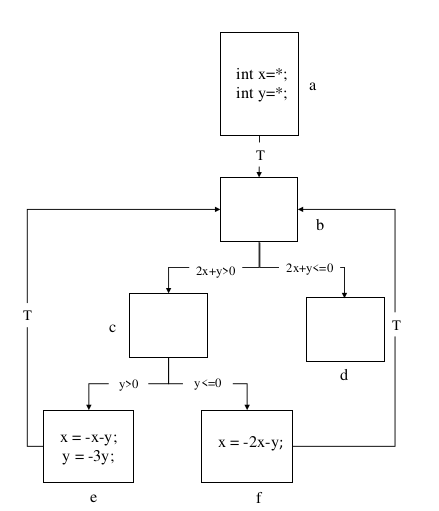
\includegraphics[scale=0.37]{1cfg.png}
\end{center}

Loop paths: $\sigma_1 = (b,c,e,b), \sigma_2 = (b,c,f,b), \sigma_3 = (b,d)$
\end{frame}

\begin{frame}\frametitle{Path Dependency Automaton}
\begin{definition}[Path Dependency Automaton(PDA)]
Given a loop with CFG $\mathcal{G}$, the path dependency automaton of this loop is $\mathcal{A} = (S,T, init, accept)$ where 
\begin{itemize}
\item $S$ is the set of states. Each $\sigma \in S$ corresponds to a path in the loop.
\item $T \subseteq S \times S $ is a set of transistions. $(\sigma_i, \sigma_j)\in T$ means that $\exists n > 0$ s.t. $\theta(\sigma_j, \mathcal{V}_{\sigma_i}^n) = true\wedge tail(\sigma_i) = head(\sigma_j)$.
\item $init, accept$ are the set of initial states and accepting states respectively.

\end{itemize}
\end{definition}
\end{frame}

\begin{frame}\frametitle{Example}
\begin{center}
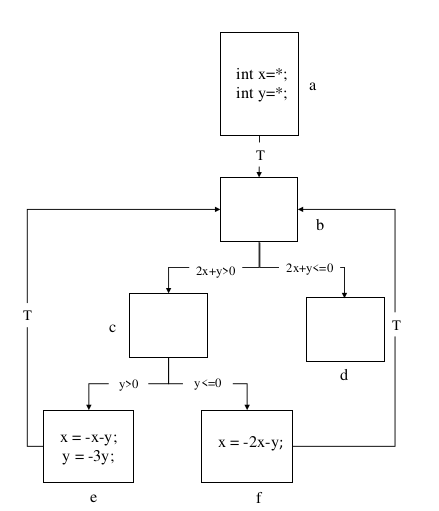
\includegraphics[scale=0.37]{1cfg.png}
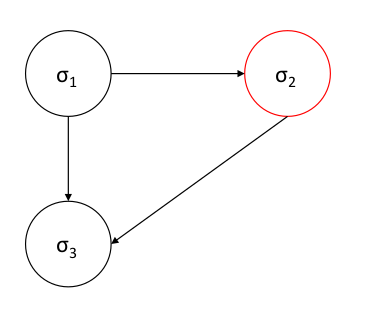
\includegraphics[scale=0.3]{1pda.png}
\end{center}
\end{frame}
\begin{frame}\frametitle{Overview of \textsc{MLTerm}}

\begin{center}
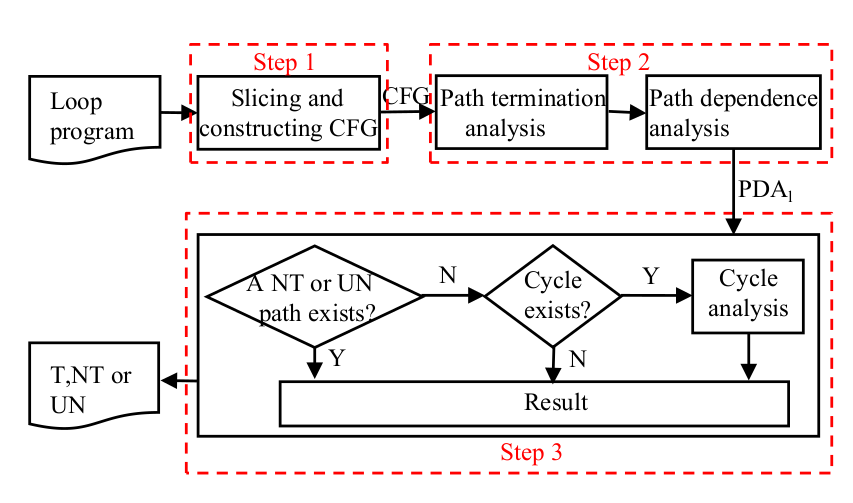
\includegraphics[scale=0.3]{overview.png}	

\end{center}

The main part of termination analysis is step 3, where we first check if there is NT or UN path reachable. If not, do cycle analysis.
\end{frame}


\begin{frame}\frametitle{Path Termination Analysis}
\begin{multicols}{2}
If the path is not iterative, it is terminating.

Otherwise the path represents a loop.
\[while(Bx > 0)\{x = Ax\}\]

Do termination analysis on this loop and output $T$ if it is terminating.

The method for the terminating analysis is from [Tiwari].

{\tiny[Tiwari] Termination of Linear Program.}
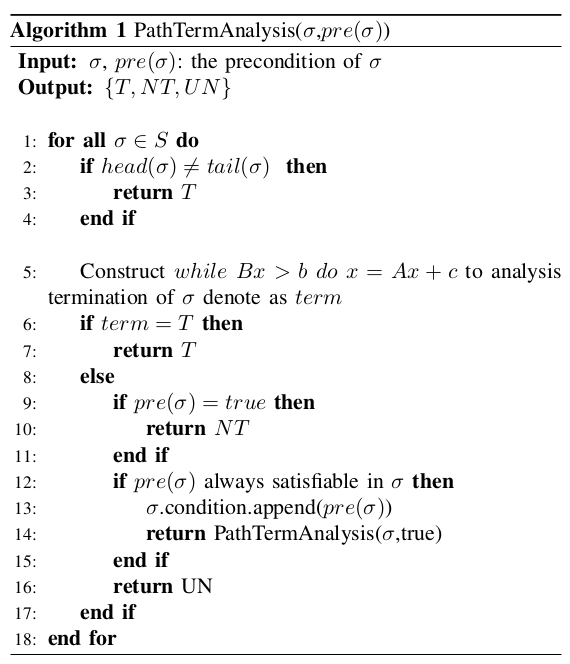
\includegraphics[scale=0.3]{algo1.png}

\end{multicols}
\end{frame}

\begin{frame}\frametitle{Examples}
\begin{center}
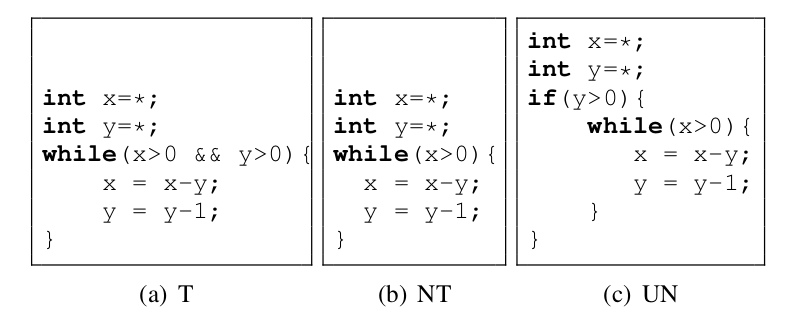
\includegraphics[scale=0.35]{algo1Exp.png}

(b) NT with witness $x = 2, y = 1$.
(c) $pre(\mathcal{G})$ is not always satisfied.
\end{center}
\end{frame}
\begin{frame}\frametitle{Path Dependece Analysis}
\begin{multicols}{2}
Target of path dependence anaylysis is to determine whether a loop path can transit to another.

There are two kinds of transitions:
\begin{itemize}
\item $\sigma_i$ is terminating and its outdegree is $1$.

\item Check whether the formula $\exists n. \theta(\sigma_j, \mathcal{V}^n_{\sigma_i})$ is $true$.
\end{itemize}

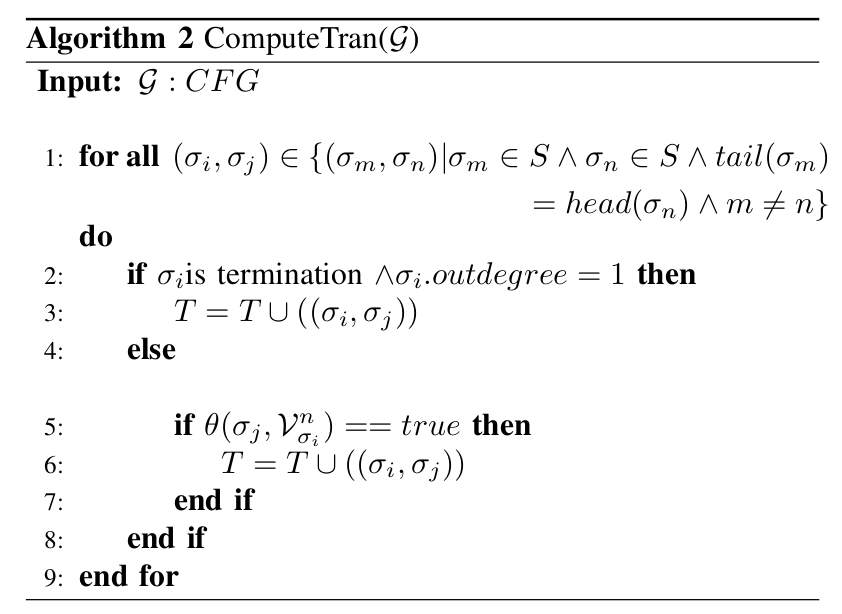
\includegraphics[scale=0.2]{algo2.png}
\end{multicols}
\end{frame}


\begin{frame}\frametitle{Cycle Analysis}
\begin{definition}[Cycle in PDA]
Let $\mathcal{C}=\{\sigma_1, \sigma_2, \ldots, \sigma_\}$. $\mathcal{C}$ is a cycle of PDA  if
\begin{itemize}
\item $\mathcal{C} \subset S$
\item $\sigma_1, \sigma_2,\ldots, \sigma_n$ constitues an SCC in PDA.
\end{itemize}
\end{definition}
Classify cycles into 2 categories:
\begin{itemize}
\item Type 1 cycle:
All path in $\mathcal{C}$ are one-time paths. 
\item Type 2 cycle: Otherwise.
\end{itemize}
\end{frame}

\begin{frame}\frametitle{Cycle Analysis for Type 1}
Idea: Since all paths are simple, we can simply merge them into a new path and do path termination analysis on the new path.
\begin{center}
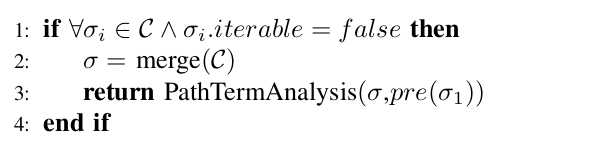
\includegraphics[scale=0.4]{type1cyclealgo.png}
\end{center}
\end{frame}
\begin{frame}\frametitle{Cycle Analysis for Type 2}
\begin{center}
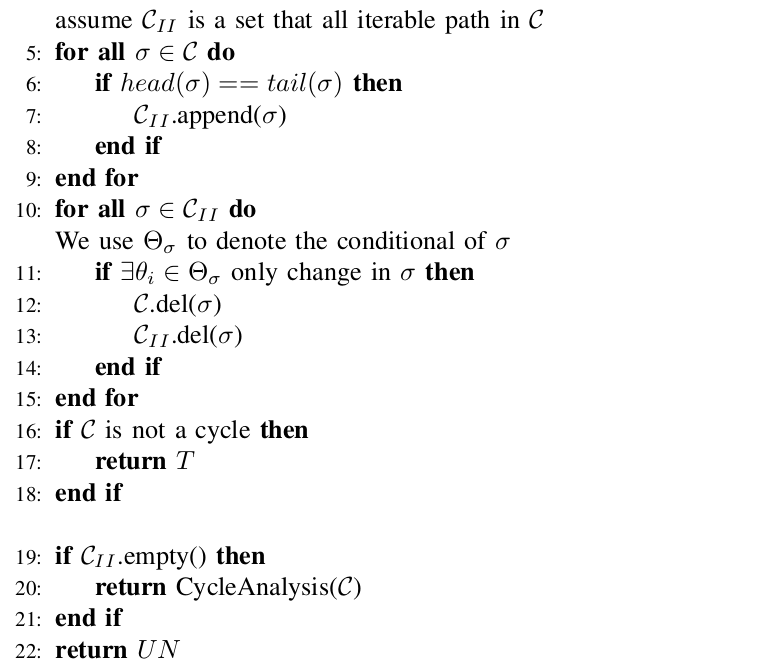
\includegraphics[scale=0.3]{type2cyclealgo.png}
\end{center}
\end{frame}

\begin{frame}\frametitle{Experimental Results}
\begin{center}
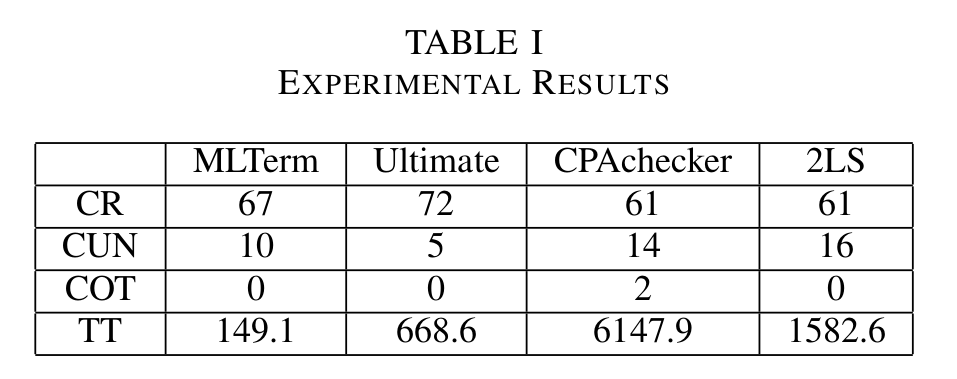
\includegraphics[scale=0.3]{general.png}
\end{center}
Benchmark: SV-COMP 2020

CR: num of right result. 

CUN: num of unknown.

COT: num of timeout.

TT: total time.
\end{frame}
\begin{frame}\frametitle{Experimental Results}
\begin{center}

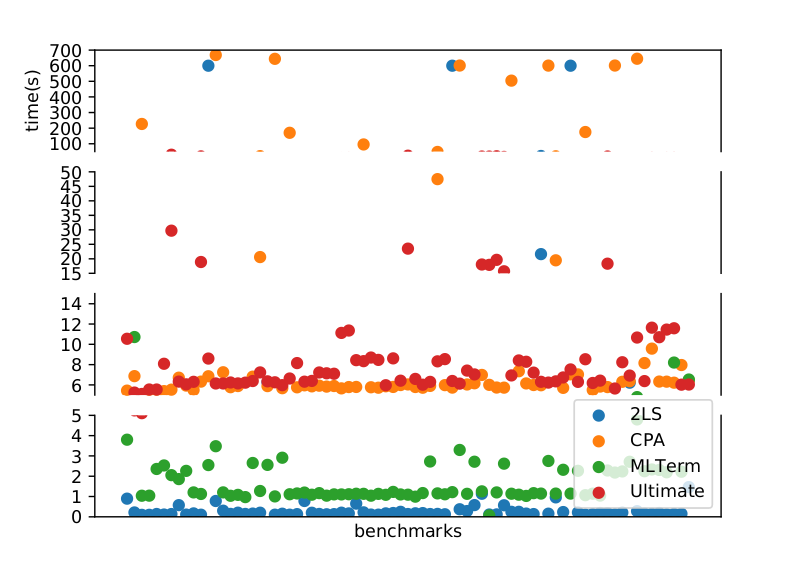
\includegraphics[scale=0.4]{detailed.png}
\end{center}
\end{frame}
\end{document}